\documentclass{article}
\usepackage[T1]{fontenc}
\usepackage{lmodern}
\usepackage{graphicx}
\usepackage{amsmath,amssymb}
\usepackage[a4paper,margin=2cm]{geometry}
\usepackage[absolute,overlay]{textpos}
\setlength{\TPHorizModule}{1mm}
\setlength{\TPVertModule}{1mm}
\usepackage[indonesian]{babel}
\usepackage{hyperref}
\setlength{\emergencystretch}{2em}
% unit: Halaman 51

\begin{document}

% === Halaman 51 (llm) ===

\begin{center}
\textbf{\large Man-in-the-middle-attack}\\
Serangan aktif yang berbahaya
\end{center}

\vspace{10mm}

% deskripsi: Diagram yang mengilustrasikan cara kerja serangan Man-in-the-Middle (MITM), menunjukkan interupsi koneksi asli antara User/Victim dan Web Application oleh penyerang (Man in the Middle).
% bbox normalisasi: [0.1700, 0.2600, 0.8900, 0.8500]
\begin{textblock*}{151.20mm}(35.70mm,77.22mm)
\noindent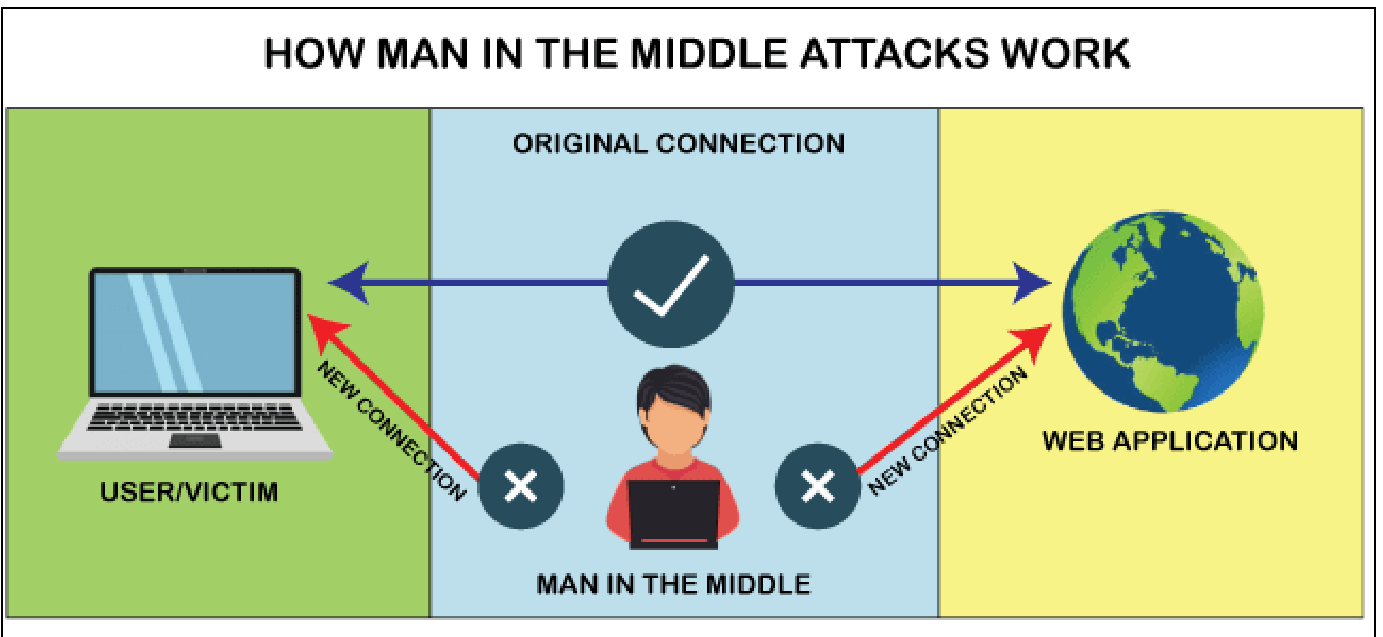
\includegraphics[width=151.20mm,height=175.23mm]{../../images/llm/page_051_img_01.png}%
\end{textblock*}

\end{document}
